% =============================================================================
% Figure blocks for the GuIA papers. Generated figures live in eval/figures/
% as both .png and .pdf (vector).
%
% PLACEMENT: \includegraphics uses BARE filenames (no folder, no extension),
% matching the existing convention in the papers (e.g. {number_of_visitors},
% {location}). Upload the image files to the SAME location where your other
% figures already live (the Overleaf project root). LaTeX picks the .pdf over
% the .png automatically when both are present; upload whichever you prefer.
% If you keep images in a subfolder instead, add \graphicspath{{figs/}} in the
% preamble rather than editing every path here.
%
% EXACT POSITION: the figures use [H] (not [h]) so each one is placed EXACTLY
% where this block sits in the text, with no floating to another page. [H]
% needs \usepackage{float} in the preamble. Paper B ("Towards Adaptive...")
% already loads it; for Paper A ("Renaixement...") add \usepackage{float} to
% the preamble. (If you ever prefer to let a figure float, change its [H] back
% to [htbp].)
%
% Numbers in the captions are read from the real eval runs (see
% eval/make_figures.py). Captions are written in two registers: PAPER A is the
% technical/working-paper version, PAPER B the social-innovation version.
% =============================================================================


% #############################################################################
% PAPER A  —  "Renaixement Museum Interactive Audioguide" (technical)
% #############################################################################

% --- A1 : faithfulness by question bucket -----------------------------------
\begin{figure}[H]
\centering
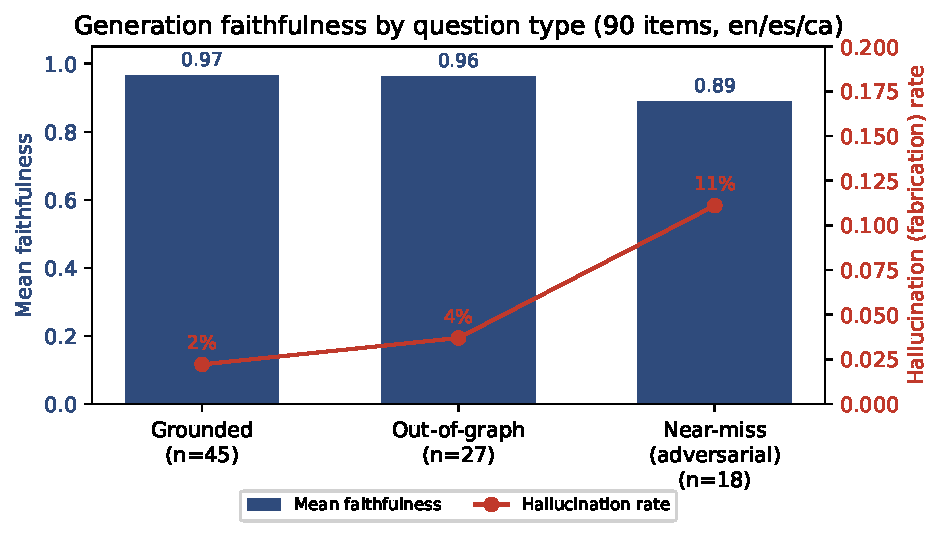
\includegraphics[width=1\linewidth]{faithfulness_by_bucket}
\caption{Generation faithfulness by question type (90 items across English,
Spanish, and Catalan). Bars show mean faithfulness; the line shows the
fabrication (hallucination) rate on the right axis. Faithfulness stays high for
grounded and out-of-graph questions and drops only for the adversarial near-miss
probes, where the few fabrications concentrate.}
\label{fig:faithfulness_bucket}
\end{figure}

% --- A2 : prompt sensitivity per axis ---------------------------------------
\begin{figure}[H]
\centering
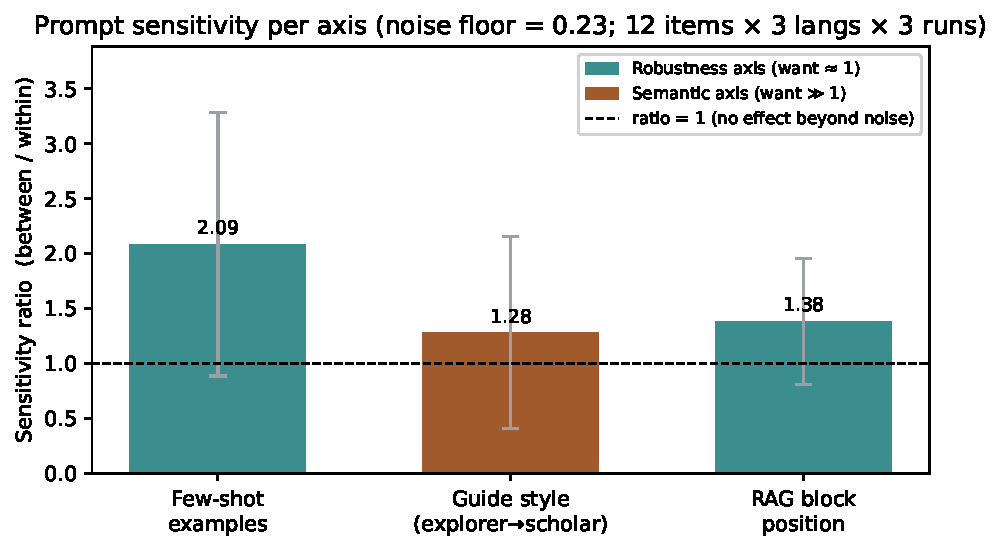
\includegraphics[width=1\linewidth]{prompt_sensitivity}
\caption{Prompt sensitivity per axis (12 grounded questions $\times$ 3 languages
$\times$ 3 runs). The sensitivity ratio is the divergence between a prompt
variant and the baseline divided by the divergence between identical runs of the
baseline (the noise floor, $0.23$); error bars are one standard deviation. A
ratio near one (dashed line) means the change moved the answer no more than
resampling noise. Removing the few-shot examples has the largest effect, while
moving the retrieved-context block is close to neutral.}
\label{fig:prompt_sensitivity}
\end{figure}

% --- A3 : prompt sensitivity per axis, by language --------------------------
\begin{figure}[H]
\centering
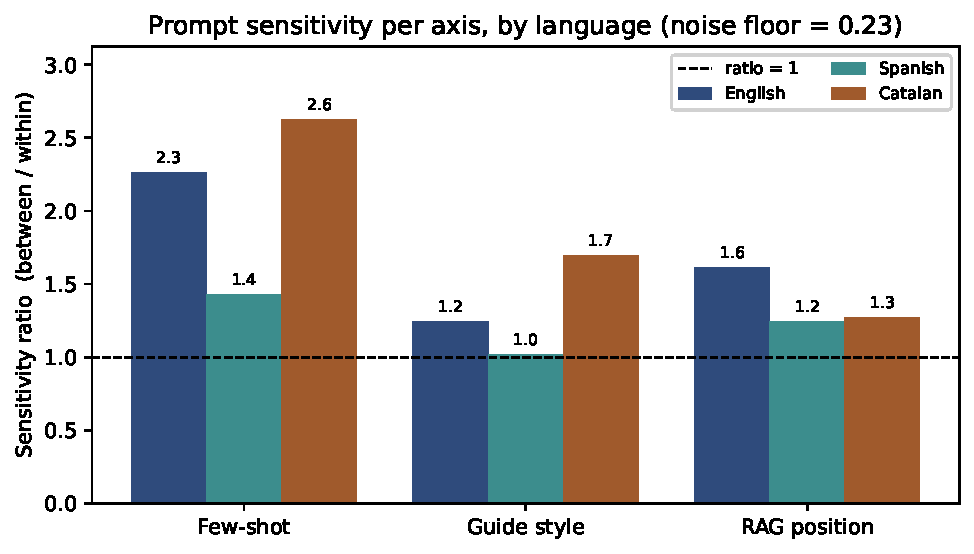
\includegraphics[width=1\linewidth]{prompt_sensitivity_by_lang}
\caption{Prompt sensitivity per axis, broken down by language. The ordering of
the effects is consistent across English, Spanish, and Catalan: the few-shot
examples are the most influential component in every language, which indicates
the effect is a property of the prompt rather than an artefact of a single
language.}
\label{fig:prompt_sensitivity_lang}
\end{figure}

% --- A4 : faithfulness verdict mix by language ------------------------------
\begin{figure}[H]
\centering
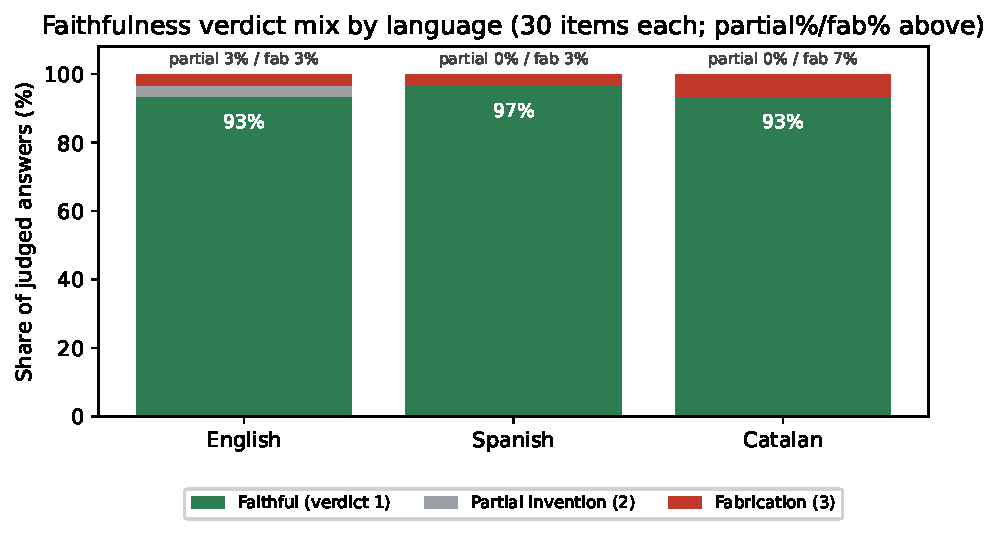
\includegraphics[width=1\linewidth]{verdicts_by_language}
\caption{Faithfulness verdict mix by language (30 items each). Each bar is the
share of judged answers rated faithful, partially invented, or fabricated; the
partial and fabrication percentages are printed above each bar. The faithful
share stays between 93\% and 97\% across the three languages, indicating
consistent grounding behaviour regardless of the answering language.}
\label{fig:verdicts_lang}
\end{figure}


% #############################################################################
% PAPER B  —  "Towards Adaptive and Situated AI..." (social innovation)
% #############################################################################

% --- B1 : cultural attribution gap (eurocentric fingerprint) ----------------
\begin{figure}[H]
\centering
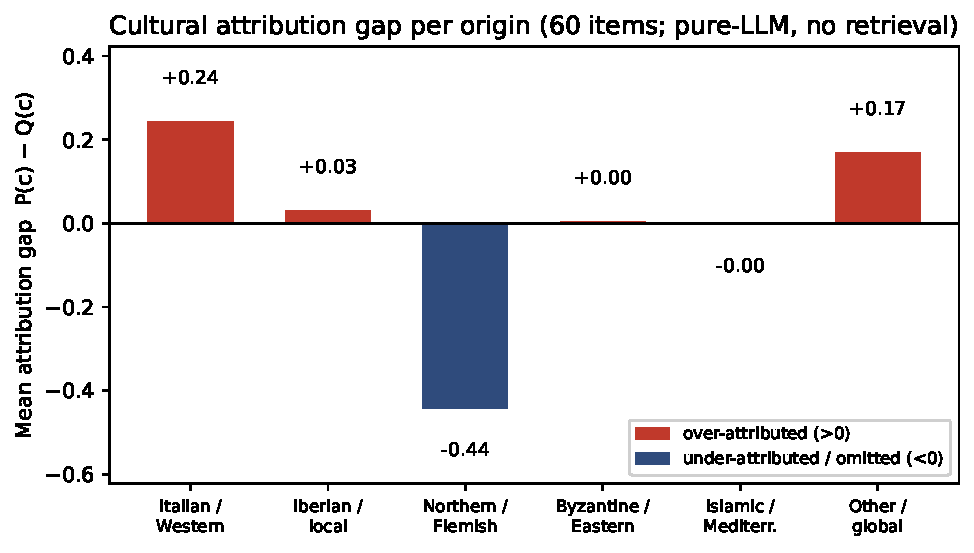
\includegraphics[width=1\linewidth]{cultural_gap}
\caption{Mean cultural attribution gap $P(c)-Q(c)$ per origin (60 items, answered
without retrieval to isolate the model's own assumptions). Positive bars mark
cultural origins the guide over-attributes; negative bars mark origins it
under-attributes or omits. The guide systematically over-weights the
Italian/Western lens and under-represents the Northern/Flemish background of the
works.}
\label{fig:cultural_gap}
\end{figure}

% --- B2 : retrieval recall by category --------------------------------------
\begin{figure}[H]
\centering
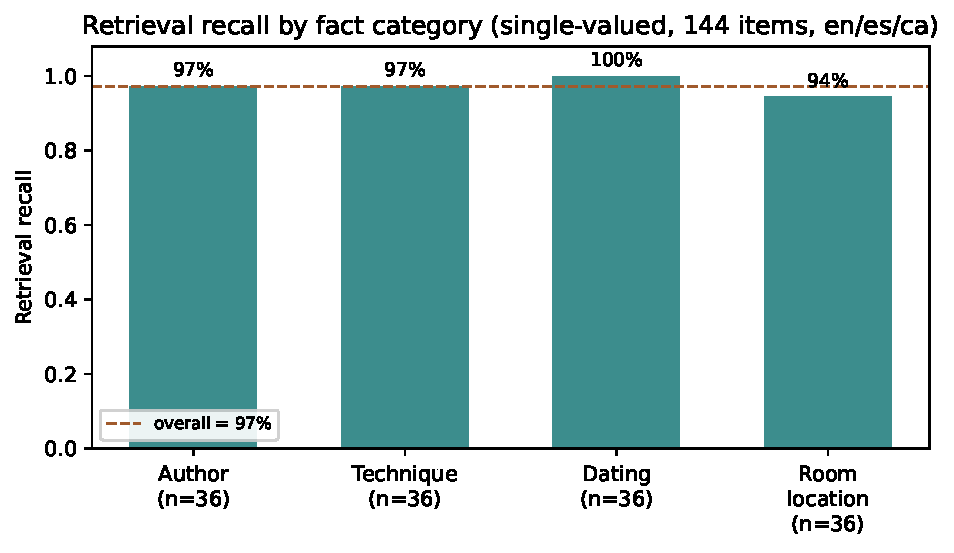
\includegraphics[width=1\linewidth]{retrieval_recall}
\caption{Retrieval recall by fact category for single-answer questions (144 items
across the three languages). The system recovers the correct author, technique,
dating, or room of a work in around 97\% of cases (dashed overall line), showing
that the right fact is usually fetched from the Knowledge Graph before the answer
is generated.}
\label{fig:retrieval_recall}
\end{figure}

% --- B3 : Cultural Bias Score by artist origin ------------------------------
\begin{figure}[H]
\centering
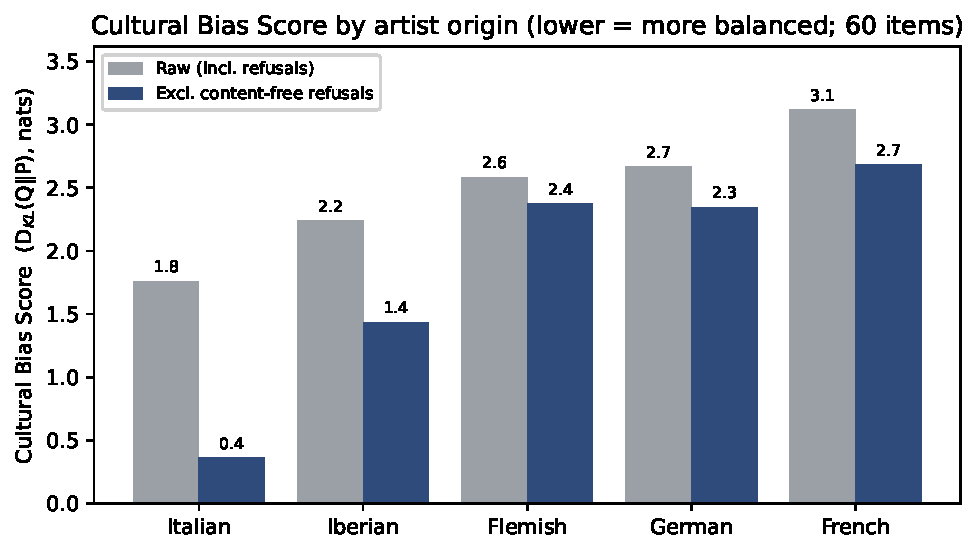
\includegraphics[width=1\linewidth]{cbs_by_origin}
\caption{Cultural Bias Score $D_{KL}(Q\,\|\,P)$ by artist origin (60 items; lower
is more balanced), shown both raw and with content-free refusals excluded. Works
of Italian origin are described most accurately, while Flemish, German, and French
works diverge most from their reference, confirming that non-Italian traditions
are flattened more often.}
\label{fig:cbs_origin}
\end{figure}

% --- B4 : Cultural Bias Score by language -----------------------------------
\begin{figure}[H]
\centering
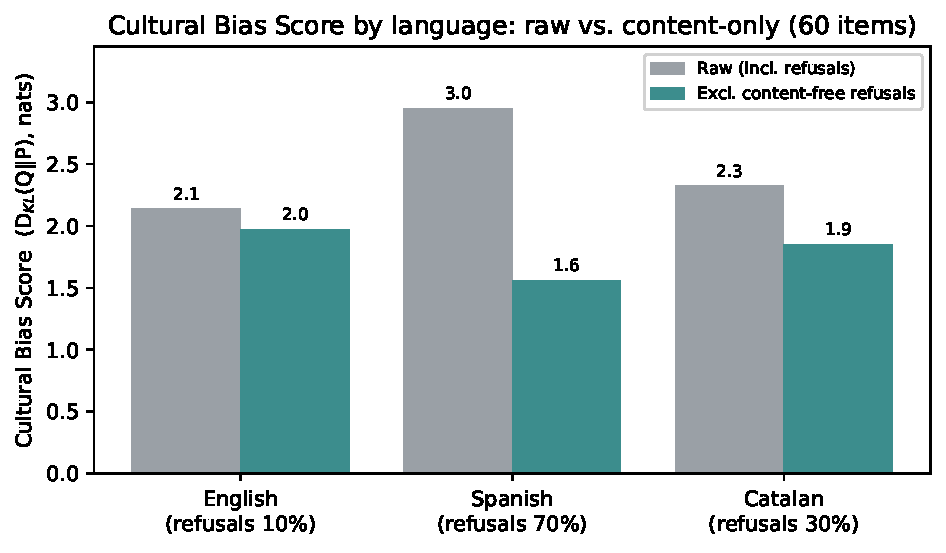
\includegraphics[width=1\linewidth]{cbs_by_language}
\caption{Cultural Bias Score by language, raw versus excluding content-free
refusals (60 items; the refusal rate is noted under each language). Without
museum context the guide often declines to answer, most frequently in Spanish,
which inflates the raw score; once only substantive answers are counted Spanish
is in fact the most balanced of the three. Working in several languages does not
by itself guarantee a fair cultural framing.}
\label{fig:cbs_language}
\end{figure}
